% BPA construction cutaway (Chapter 7, sec:fw_bpa).
% Compile: pdflatex -output-directory=.. bpa_construction.tex
\documentclass[border=6pt]{standalone}
\usepackage[T1]{fontenc}
\usepackage{mathpazo}
\usepackage{tikz}
\usetikzlibrary{arrows.meta, calc, decorations.pathmorphing}
\begin{document}
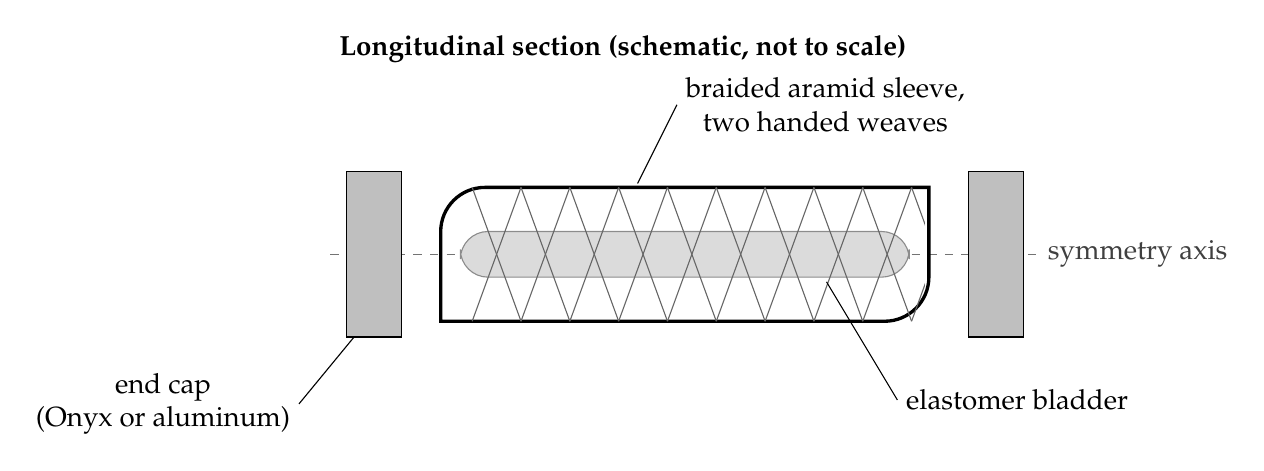
\begin{tikzpicture}[
  font=\normalsize,
  lab/.style={align=center, inner sep=3pt},
  leader/.style={-, thin},
]

% Geometry: actuator spans x 2.2..9.4, half-height 0.85, midline y=0
\def\Xo{2.35} \def\Xi{9.25}   % sleeve outer x-limits
\def\Bo{-0.5}  \def\Bt{0.5}   % bladder half-height

% Symmetry axis
\draw[dashed, black!55] (1.3,0) -- (10.3,0) node[lab, anchor=west, black!75] {symmetry axis};

% Bladder
\fill[black!14, rounded corners=10pt] (\Xo+0.6,\Bo*0.58) rectangle (\Xi-0.6,\Bt*0.58);
\draw[black!45, rounded corners=10pt] (\Xo+0.6,\Bo*0.58) rectangle (\Xi-0.6,\Bt*0.58);

% Sleeve outline
\draw[very thick] (\Xo+0.35,-0.85) {[rounded corners=16pt] -- (\Xo+1.15,-0.85)}
  -- (\Xi-1.15,-0.85) {[rounded corners=16pt] -- (\Xi-0.35,-0.85)}
  -- (\Xi-0.35,0.85) {[rounded corners=16pt] -- (\Xi-1.15,0.85)}
  -- (\Xo+1.15,0.85) {[rounded corners=16pt] -- (\Xo+0.35,0.85)} -- cycle;

% Braid: two handed weaves, clipped to the sleeve body
\begin{scope}
  \clip (\Xo+0.4,-0.85) rectangle (\Xi-0.4,0.85);
  \foreach \i in {0,...,10} {
    \pgfmathsetmacro{\x}{\Xo+0.75+\i*0.62}
    \draw[thin, black!60] (\x,-0.85) -- (\x+0.62,0.85);
    \draw[thin, black!60] (\x,0.85) -- (\x+0.62,-0.85);
  }
\end{scope}

% End caps
\foreach \xc in {1.85, 9.75} {
  \fill[black!25] (\xc-0.35,-1.05) rectangle (\xc+0.35,1.05);
  \draw (\xc-0.35,-1.05) rectangle (\xc+0.35,1.05);
}

% Leader labels
\draw[leader] (5.2,0.9) -- (5.7,1.9) node[lab, anchor=west] {braided aramid sleeve,\\two handed weaves};
\draw[leader] (7.6,-0.35) -- (8.5,-1.85) node[lab, anchor=west] {elastomer bladder};
\draw[leader] (1.6,-1.05) -- (0.9,-1.9) node[lab, anchor=east] {end cap\\(Onyx or aluminum)};
\node[lab, anchor=west, font=\normalsize\bfseries] at (1.3,2.6)
  {Longitudinal section (schematic, not to scale)};

\end{tikzpicture}
\end{document}
